% Tento soubor nahraďte vlastním souborem s obsahem práce.
%=========================================================================
% Autoři: Michal Bidlo, Bohuslav Křena, Jaroslav Dytrych, Petr Veigend a Adam Herout 2019

% Pro kompilaci po částech (viz projekt.tex), nutno odkomentovat a upravit
%\documentclass[../projekt.tex]{subfiles}
%\begin{document}

\chapter{Úvod}
%cca strana

\chapter{Použitý Hardware}
Celá práce je implementována nad existujícím hardwarem. Konkrétně se jedná o stavebnici Adeept AWR 4WD. Její součástí jsou všechny použité motory, serva, čidla a další periferie. Mozkem, na kterém poběží software zajišťující ovládání těchto komponent, bude mikropočítač Raspberry Pi 4.

\section{HW Technologie}
Nejprve budou představeny obecné hardwarové technologie které jsou následně využívány některými z představovaných periferií.

\subsection*{Pulzně šířková modulace}
Jedná se o techniku, která umožňuje vytvořit pseudo-analogový výstup s použitím číslicových výstupů. Mikrokontroléry jsou digitální zařízení a chtěly by tedy s okolním světem komunikovat pomocí jedniček a nul. Reálný svět tak ovšem nefunguje a proto je často potřeba převádět výstup z mikrokontroléru na analogový signál. Problém je v tom, že převod digitálního signálu na analogový je relativně dlouhá a neefektivní operace. Proto vznikla pulzně šířková modulace (PWM), která umožňuje relativně jednoduše simulovat analogový výstup. \cite{embeded_robotics}

PWM využívá toho, že člověk nedokáže rozpoznat rychlé změny, například led dioda blikající na frekvenci 5000 Hz se člověku jeví jako by svítila permanentně. Mechanická zařízení také mívají relativně velkou latenci a dc motoru tedy nevadí, že místo konstantního analogového napětí dostává periodický číslicový signál. \cite{embeded_robotics}

\begin{figure}[h!]
	\centering
	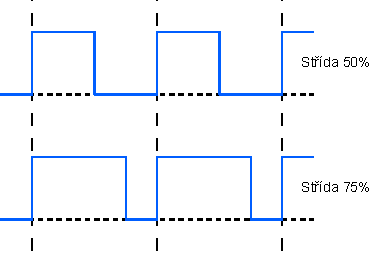
\includegraphics[scale=1]{obrazky-figures/pwm_duty_cycle.pdf}
	\caption{PWM signál pro různé hodnoty střídy}
	\label{}
\end{figure}

Při pohledu na klasický digitální signál který rovnoměrně střídá vysokou a nízkou úroveň by šlo říci, že se jedná o PWM signál se střídou 50\%. Střída (duty cycle) udává poměr času, kdy je signál v logické jedničce, ku času, kdy je v nule. Součet těchto hodnot se musí rovnat délce jedné periody. Úpravou tohoto poměru lze simulovat analogový signál. \cite{embeded_robotics}

\subsection*{I2C}
Je synchronní sběrnice, která se vyznačuje svou jednoduchostí a nízkou cenou. Využívá dva vodiče SDA (serial data) a SCL (serial clock). Oba vodiče jsou připojeny k napájecímu napětí pomocí pull-up rezistoru a bez vlivu jiného hardwaru tedy zůstávají v logické jedničce. Zařízení, která jsou na tuto sběrnici připojeny, využívají open drain k úpravě aktuální napěťové úrovně. I2C pracuje s dvěma druhy zařízení, master a slave. Master zahajuje, řídí a ukončuje komunikaci na vodiči SDA a po dobu průběhu komunikace generuje hodinový signál na SCL. Typicky se jedná o mikrokontroler. Slave jsou pak ostatní zařízení s nimiž může master komunikovat, typicky různé periferie. \cite{embeded_robotics}

\begin{figure}[h!]
	\centering
	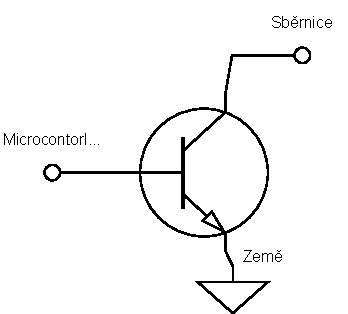
\includegraphics[scale=1]{obrazky-figures/open_drain.pdf}
	\caption{Open drain}
	\label{}
\end{figure}

Přenos jednoho datového rámce zahájí master zařízení přivedením datové sběrnice do nuly. Následující komunikace se skládá z odeslání rámce o délce osmi bitů a potvrzení o úspěšném přenosu dat od přijímajícího zařízení. Toto potvrzení se nazývá ACK a je provedeno podržením datové sběrnice v hodnotě nula po dobu jednoho taktu. Opačný stav se nazývá NACK a indikuje že nastala chyba. Ukončení přenosu je provedeno navrácením datové sběrnice na hodnotu jedna. \cite{um10204}

\begin{figure}[h!]
	\centering
	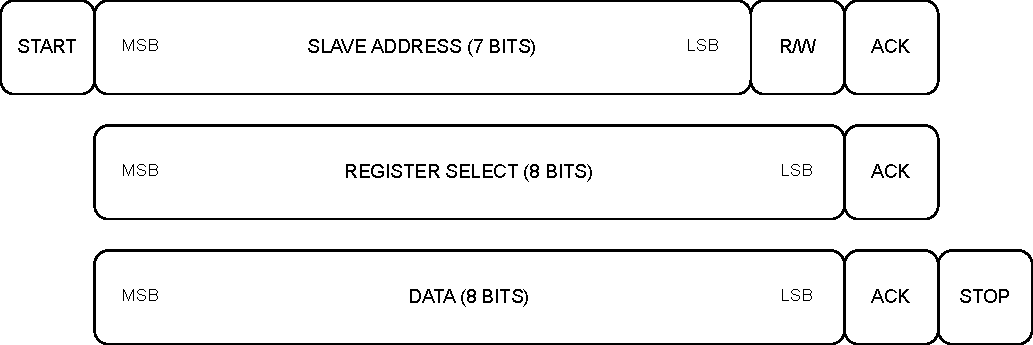
\includegraphics[scale=0.75]{obrazky-figures/i2c_data_word.pdf}
	\caption{Datové slovo sběrnice I2C}
	\label{}
\end{figure}

Na obrázku lze vidět, jak může vypadat přenos jednoho datového slova. V prvním rámci je přenesena sedmi bitová adresa, identifikující slave zařízení se kterým chce máster navázat komunikaci. Osmý bit datového rámce indikuje směr, kterým budou posílány data. V druhém rámci dojde k adresaci konkrétního registru na slave zařízení. A ve třetím, případně dalších, již probíhá samotné posílání dat mezi zařízeními. \cite{an4481}

\section{Adeept AWR 4WD}
Pohyb tohoto robota zajišťují čtyři pevná kola a zatáčení je tedy realizováno diferenciálním způsobem. To znamená, že jednotlivá kola se mohou otáčet svou vlastní rychlostí a zpomalením kol na jedné straně oproti té druhé lze provést zatáčení robota. Velkou výhodou tohoto přístupu je možnost otáčení robota na místě. Nevýhodou pak budou složitější výpočty při potřebě zahnout o nějaký přesně daný úhel.

\noindent Následující stránky popisují jednotlivé komponenty tohoto robota.

\subsection*{Robot HAT}
HAT(hardware attached on top) je hardwarová deska, která slouží k rozšíření mikrokontroléru o další funkcionalitu. Tato konkrétní se k Raspberyy Pi připojuje pomocí GPIO(General purpuse input outpu) pinů. Deska jako taková obsahuje rozšiřující čipy a rozhraní sloužící k ovládání připojených periferií.

\begin{itemize}
	\item{PCA9685 \cite{pca9685}}
	\begin{itemize}
		\item{generátor PWM signálu}
		\item{16 kanálů}
		\item{12 bitů rozlišení střídy (4096 možných hodnot)}
		\item{je ovládaný přes I2C sběrnici}
	\end{itemize}
	\item{L298P \cite{l298}}
	\begin{itemize}
		\item{ovladač pro řízení dc motoru}
		\item{základem je full bridge obvod}
		\item{umožňuje roztočit motor oběma směry}
		\item{pomocí PWM lze ovládat rychlost motorů}
		\item{připojuje motor na externí napájení}
	\end{itemize}
	\item{další rozhraní pro připojení periferií (sledování čáry, ultrazvukový senzor, led)}
\end{itemize}

\begin{figure}[h!]
	\centering
	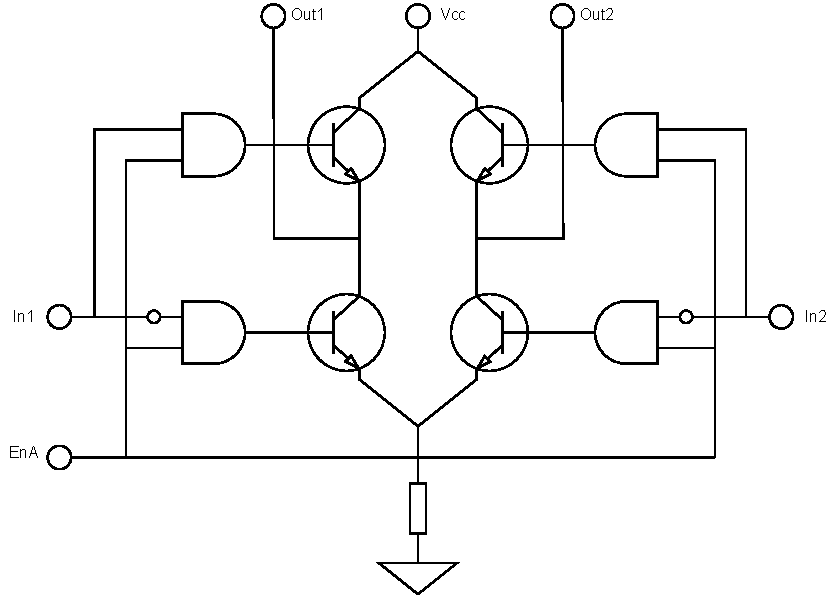
\includegraphics[scale=0.75]{obrazky-figures/motor_full_bridge.pdf}
	\caption[Full bridge ovladač motoru.]{Full bridge konfigurace pro ovládání motoru. In1 a In2 určují směr otáčení. EnA je PWM signál určující rychlost otáčení. \cite{l298}}
	\label{}
\end{figure}

\newpage
\subsection*{DC Motor}
Pohyb celého autíčka zajišťují čtyři stejnosměrným proudem(direct current) napájené motory. Ovladač motorů L298P je umístěný na Robot HAT.

\begin{figure}[h!]
	\centering
	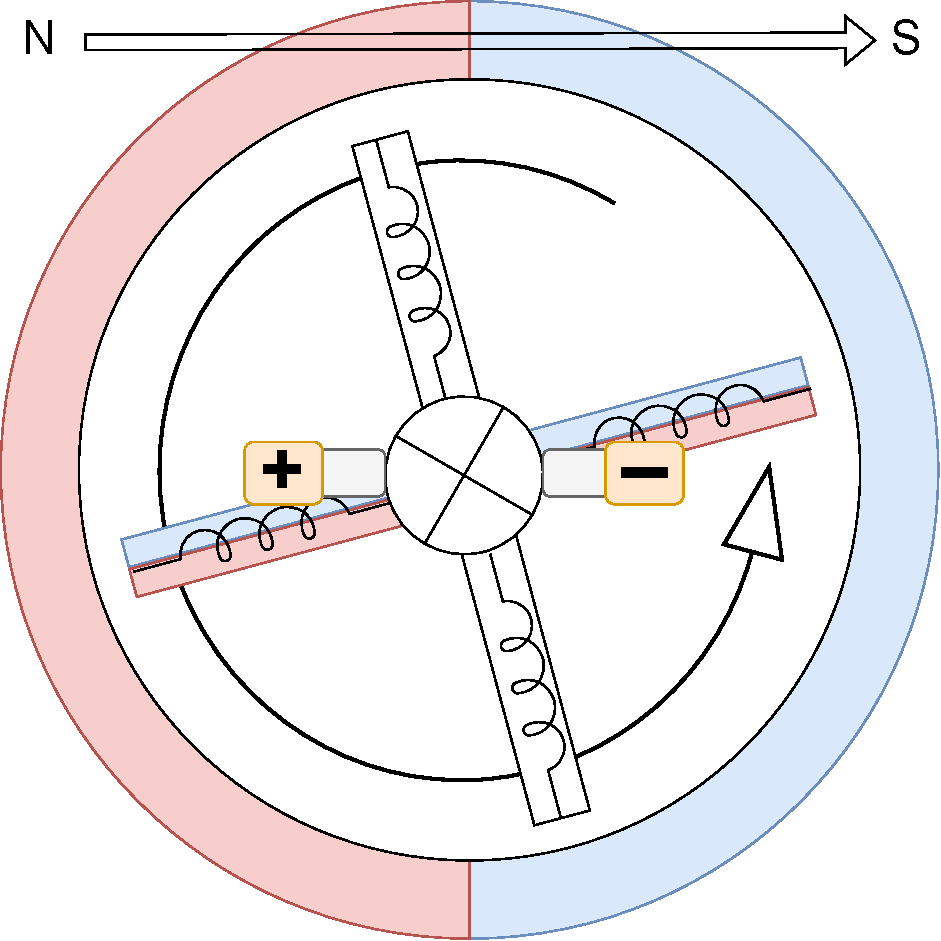
\includegraphics[scale=0.50]{obrazky-figures/dc_motor.pdf}
	\caption{Schéma DC motoru}
	\label{}
\end{figure}

Elektrický DC motor se skládá ze dvou hlavních částí, stator a rotor. Stator je statická, vnější část, a typicky se jedná o permanentní magnet. Uvnitř statoru se pak nachází rotor, ten se skládá z elektromagnetů, které při zapnutí reagují se statorem(opačné póly se přitahují a stejné odpuzují) a dojde tak k částečnému pootočení. Při správném spínání a vypínání těchto elektromagnetů lze motor rozběhnout. 
Toto střídání zajišťuje prstenec zvaný komutátor. Komutátor je rozdělen na několik od sebe odizolovaných částí, ke kterým jsou připojeny vývody elektromagnetů. S povrchem prstence jsou pomocí pružin v kontaktu dva kartáče. Tyto kartáče se již neotáčí a mohou tak být připojeny na zdroj napájení a zem. Komutátor se otáčí společně s rotorem a při tomto pohybu se kartáče postupně dotýkají různých částí komutátoru a spínají tak jednotlivé elektromagnety, ty zajistí pootočení rotoru a sepnutí následujícího magnetu. \cite{dc_motor}

\subsection*{Servo}
Servo je komponenta na první pohled podobná DC Motoru. Na rozdíl od něj se však neotáčí celých 360 stupňů, ale bývá omezena na nějakou menší hodnotu, například 180 stupňů. Hlavním výhodou a důvodem pro použití serva je plná kontrola nad úhlem natočení jeho hřídele. \cite{embeded_robotics}

\begin{figure}[h!]
	\centering
	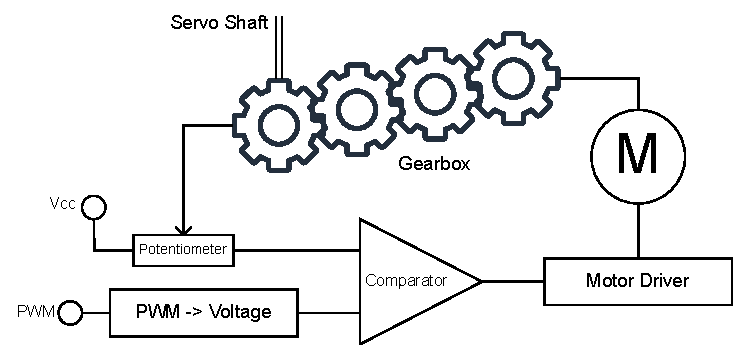
\includegraphics[scale=0.9]{obrazky-figures/servo.pdf}
	\caption{Vnitřní zapojení serva}
	\label{}
\end{figure}

Při pohledu na vnitřní zapojení serva lze zjistit, že se prakticky jedná o klasický dc motor připojený na převodovku a rozšířený o elektroniku na jeho řízení. K nastavení úhlu serva se využívá PWM signál. Ten je první přeložený na napěťovou úroveň, která je porovnána s aktuálním natočením serva a výsledek udává směr, kterým se bude otáčet motor. Aktuální natočení serva je získáno využitím potenciometru zapojeného na výstupní hřídel serva. \cite{embeded_robotics}

Adeept AWD 4WD využívá pouze jedno servo, a to na ovládání úhlu natočení kamery. Konkrétně se jedná o model Adeept AD002. Generování PWM signálu pro ovládání zajišťuje čip PCA9685, který je součástí Robot HAT.

\subsection*{Ultrazvukový senzor hloubky}
Slouží k určení vzdálenosti mezi robotem a překážkou. Funguje na principu radaru. Vyšle ultrazvukovou vlnu na frekvenci 40Khz a uloží si časovou značku. Následně poslouchá než se mu vrátí odražená vlna a opět si uloží značku.
Pro výpočet vzdálenosti lze využít následující vzorec:

$$S = \frac{(T_2 - T_1) * V_S}{2}$$

Kde $T_1$ je moment kdy byla vyslána vlna $T_2$ kdy byla vlna přijata a $V_S$ rychlost šíření zvuku ve vzduchu (cca 340m/s). Výsledek se pak dělí dvěma, protože doba $T_2 - T_1$ je rovna času k překážce a zpět.

Konkrétně se jedná o model hc-sr04, který dokáže změřit vzdálenost od 2cm do 400cm s přesností na 3mm. Ovládání senzoru je pak realizováno pomocí dvou jeho vývodů a to trig a echo. Mikrokontroler vyšle pulz na trig vodiči. Ten zaktivuje senzor, který zahájí měření. To je realizováno osmi čtyřicetihercovými pulzy ze kterých vypočítá výslednou vzdálenost. Po dokončení výpočtu nastaví echo vodič do hodnoty jedna na dobu rovnou času mezi odesláním a zachycením ultrazvukového signálu. \cite{embeded_robotics}

\begin{figure}[h!]
	\centering
	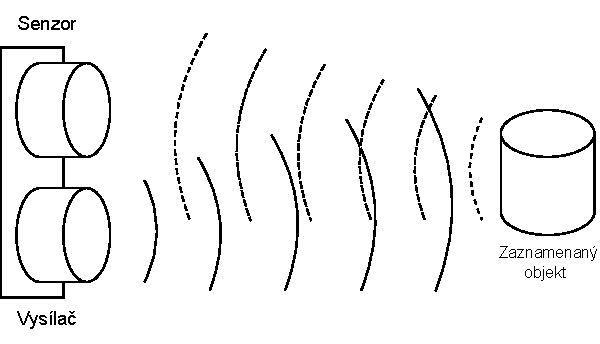
\includegraphics[scale=0.75]{obrazky-figures/ultrasonic.pdf}
	\caption{Ultrazvukový senzor}
	\label{}
\end{figure}

\subsection*{Třícestný senzor pro sledování čáry}
Modul využívá fakt, zě intenzita světla odraženého od povrchu je závislá na barvě dané plochy. Například černá barva pohltí téměř veškeré světlo, naopak bílá téměř vše odrazí. Používáno je infračervené záření, protože není ovlivněno okolními zdroji světla, odráží se od velkého množství materiálů a je přesné. Jedná se o třícestný modul a skládá se tedy ze setu tří vysílačů a senzorů. Pokud vysílač svítí a senzor nezaznamenává dostatečnou intenzitu odraženého světla, znamená to, že byla nalezena černá čára. \cite{embeded_robotics}
Komunikace s mikrokontrolerem je realizována pomocí GPIO vstupů, na které jsou připojeny tři vývody z modulu. Každý z nich reprezentuje jeden set vysílače a senzoru. Jednička na výstupu indikuje, že čára byla detekována.

\subsection*{WS2812 RGB LED}
WS2812 je druh adresovatelných LED diod. Pojmem adresovatelných je myšleno, že není každá dioda připojena k mikrokontroleru zvláště, ale sdílejí jeden datový vodič pro nastavování barev. Prakticky to znamená, že pásek, který může obsahovat i stovky diod je připojený jen pomocí tří vodičů. Těmito vodiči jsou napájení, země a vstupní data. \cite{ws2812}

\begin{figure}[h!]
	\centering
	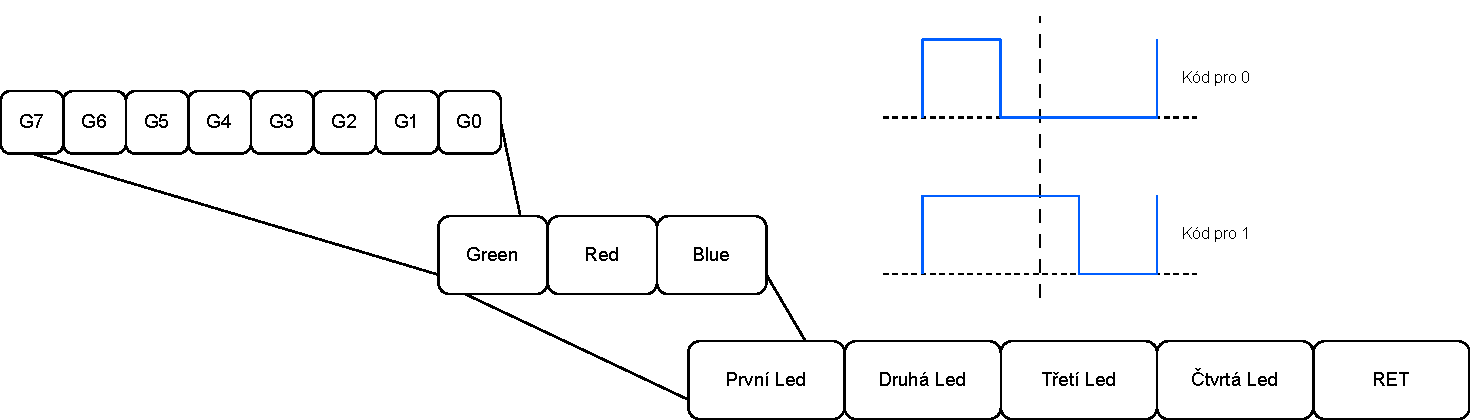
\includegraphics[scale=0.55]{obrazky-figures/ws2812_led.pdf}
	\caption{Komunikační protokol pro WS2812 led}
	\label{}
\end{figure}

Diody jsou na pásku zapojeny sériově. Každá dioda má DIN a DO port. Pokud dioda přijme data, která jí nejsou určená, přeposílá je dále. Komunikace vždy začíná klidovým stavem, datový vodič je v nule. Datové slovo se skládá z 24 bitových bloků pro každou diodu. Blok obsahuje tři osmi bitové hodnoty, jednu pro každou barevnou složku (MSB je posíláno první). Diody pak fungují tak, že přijmou prvních 24 bitů, podle kterých nastaví svou barvu. Tuto část odeberou z datového slova a zbytek přeposílají na výstup. \cite{ws2812}

\section{Raspberry Pi 4b}
Jako mozek celého systému je použit mikropočítač Raspberry Pi. V porovnání s běžně používanými mikrokontroléry, sloužícími pro řízení vestavěných systémů, se jedná o výkonnější hardware, který zvládá i komplexnější operace, jako běh plnohodnotného operačního systému a zpracování obrazu. Konkrétně se jedná o verzi 4 model B s operační pamětí o velikosti čtyř gigabajtů. Tato verze obsahuje 64bitový procesor, ten je potřeba pro spuštění 64 bitového Ubuntu serveru, který je doporučeným operačním systémem pro požití ROS2 na Raspberry Pi.
Komunikace s většinou použitých periferií je uskutečněna pomocí General Purpuse Input Output(GPIO) pinů. Jedná se o číslicové vývody, které podle potřeby můžou fungovat jako vstup i výstup ze zařízení. Některé z nich pak mají ještě speciální funkce, například GPIO 2 a 3 můžou pracovat jako SDA a SCL připojení pro I2C komunikaci.

\begin{figure}[h!]
	\centering
	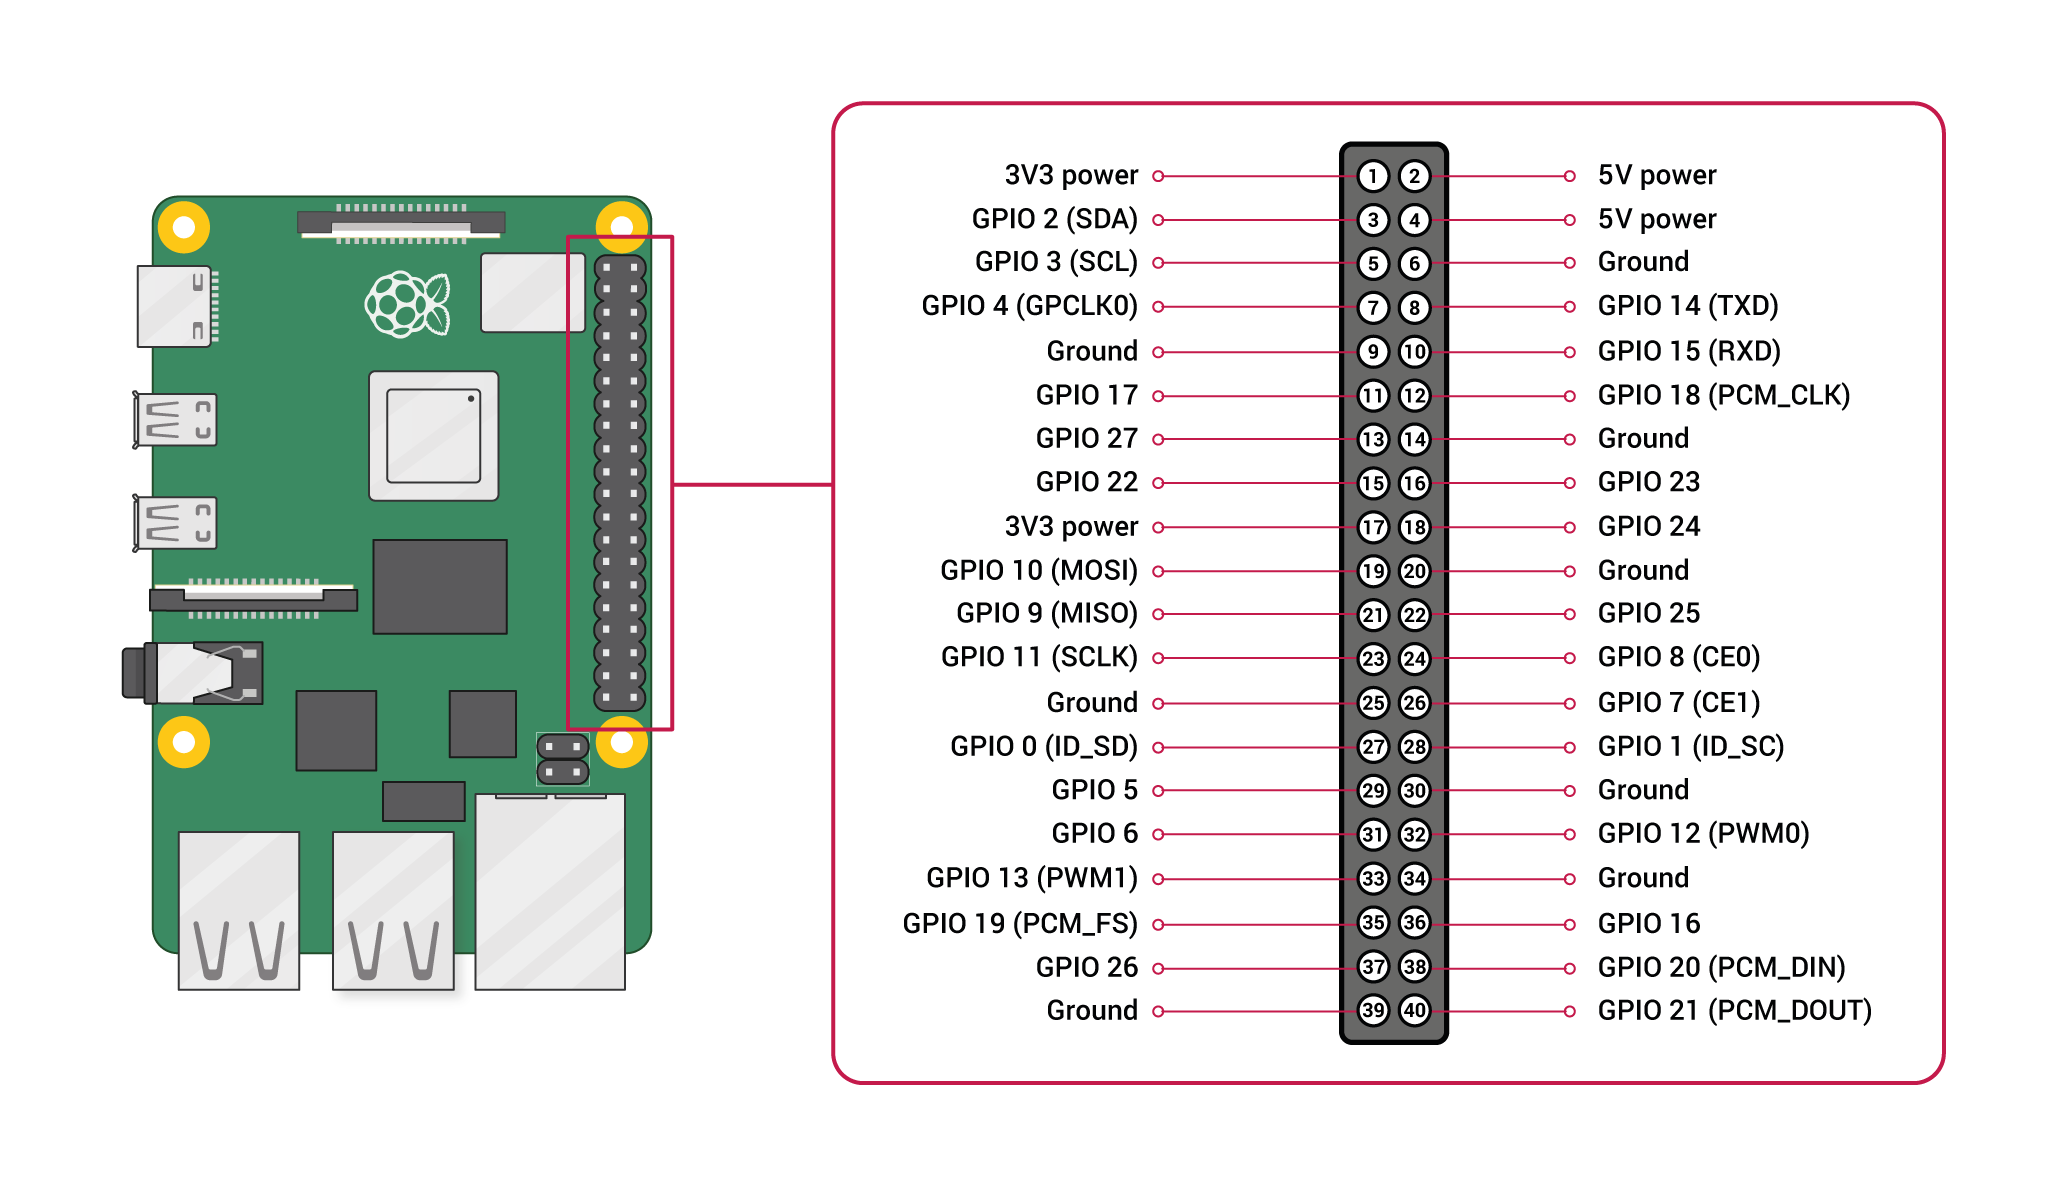
\includegraphics[scale=0.15]{obrazky-figures/gpio_pinout.png}
	\caption{GPIO pinout pro Raspberry Pi}
	\label{}
\end{figure}

\subsection*{Camera}
Přímo k rapsberry pi je připojena oficiální rpi camera v3. Tento modul dokáže nahrávat video až v rozlišení 2304 × 1296 pixelů a 56 snímcích za vteřinu. Avšak pro zpracování, případně analýzu obsahu videa v reálném čase s těmito specifikacemi nemá Raspberry Pi dostatečný výkon. Prakticky budou využity nižší rozlišení a snímkovací frekvence. \cite{rpi_camera}
%opencv

\chapter{Software pro řízení robota}
Jak už bylo řečeno, software poběží na Raspberry Pi. Jako primární programovací jazyk byl zvolen python, protože je jedním z oficiálních jazyků podporovaných ROS2 a také jsou v něm implementovány potřebné knihovny pro ovládání periferií.

\section{Aktuální software}
Robot Adeept AWR 4WD je dodáván s ukázkovým softwarem. Ten je implementován v jazyce Python a využívá knihovny třetích stran sloužící k nízkoúrovňovému ovládání hardwarových komponent. Aby byl robot responzivní je celá implementace řešena s použitím python modulů pro realizaci multithreadingu.

\section{Seznámení s ROS2}
ROS2 je middleware sloužící k vývoji a řízení robotů. Middleware je softwarová vrstva běžící nad operačním systémem. Jejím úkolem je rozšíření operačního systému o další funkcionalitu. Typickou součástí middlewaru bývají knihovny, ovladače, vývojové a monitorovací nástroje. Může také specifikovat doporučené metodologie pro vývoj. ROS2 je již druhá verze tohoto softwaru, která rozšiřuje a opravuje neduhy první verze. Původní ROS1 je považován za de-facto standart pro vývoj robotických aplikací.
Tato práce využívá ROS2 distribuci jménem iron. Distribuce v ROS2 lze popsat jako set operačního systému, knihoven a dalších aplikací, které jsou otestovány a je zaručeno, že jsou navzájem kompatibilní. Velkou výhodou ROS je fakt, že se jedná o open source projekt. Díky tomu kolem něj vznikla velká komunita vývojářů, ale i firem a dalších institucí, které tvoří mnoho souvisejícího obsahu. Existuje tedy velké množství knihoven, dokumentací a návodů které usnadňují vývojářům práci. \cite{ros2_introduction}

\subsection*{Vrstvy ROS2}
Na nejvyšší úrovni, se nachází programátor, který interaguje s klientskými knihovnami pro vývoj ROS2 aplikací. Tyto knihovny jsou oficiálně dvě a to rclpy pro python a rclcpp pro C++. Existují také implementace pro další programovací jazyky (rclc, java, C\#), které jsou však udržovány komunitně. Všechny klientské knihovny pak využívají RCL. To je jádrem celého ROS a obsahuje implementaci všech ros2 funkcionalit. Je napsáno v jazyce C a jeho součástí je rozhraní, pomocí kterého poskytuje svou funkcionalitu ostatním klientským knihovnám. Díky tomuto přístupu se uzly implementované v pythonu budou chovat stejně jako ty implementované v c++. Z toho pak také vyplývá, že uzly implementované na různých klientských knihovnách spolu mohou bez problémů komunikovat.
Poslední vrstvou je data distribution service. DDS je komunikační vrstva implementována na UDP protokolu sloužící k předávání informací mezi procesy. Má charakteristiky systémů reálného času, zajišťuje kvalitu a zabezpečení komunikace. Také umožňuje vyhledávání uzlů bez potřeby centralizovaného serveru (vyhledávání je realizováno s využitím multicastové komunikace, zprávy zasílané mezi jednotlivými uzly pak využívají klasický unicast). \cite{ros2_introduction}

\begin{figure}[h!]
	\centering
	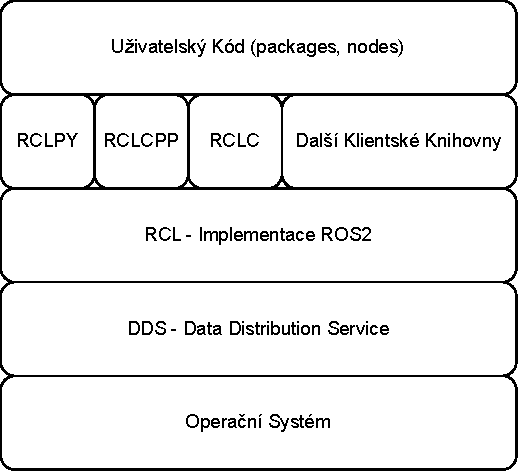
\includegraphics[scale=0.75]{obrazky-figures/ros_layers.pdf}
	\caption{Vrstvy ROS2 systému}
	\label{}
\end{figure}

\subsection*{Vývoj v ROS2}
Nejvyšší organizační jednotkou v ROS2 je workspace. Jedná se o složku, která slouží k organizaci zdrojových souborů, jejich instalaci a následné spouštění. ROS2 se také kvalifikuje jako workspace a před použitím musí být nejprve aktivován. K tomu v linuxu slouží příkaz \verb|source|. Aktivace workspace je akumulativní, to znamená, že v jeden moment může být aktivních několik workspace najednou. Typicky se první aktivuje základní ros2 instalace, která tvoří takzvanou underlay vrstvu. Vývojový workspace aktivovaný jako druhý, se pak nazývá overlay. Pokud má overlay nějaké závislosti, měly by být uspokojeny v underlay.
Zdrojové soubory v rámci workspace jsou pak organizovány do packages. Package může obsahovat zdrojové soubory, knihovny a definice zpráv. Packages na sobě můžou navzájem záviset (např: package která využívá interface závisí na jiné která tento interface definuje). \cite{ros2_introduction}

\begin{figure}[h]
	\begin{forest}
		for tree={
			font=\ttfamily,
			grow'=0,
			child anchor=west,
			parent anchor=south,
			anchor=west,
			calign=first,
			inner xsep=7pt,
			edge path={
				\noexpand\path [draw, \forestoption{edge}] (!u.south west) +(7.5pt,0) |- (.child anchor) \forestoption{edge label};
			},
			before typesetting nodes={
				if n=1
				{insert before={[,phantom]}}
				{}
			},
			fit=band,
			before computing xy={l=15pt},
		}
		[Workspace
			[build {\hspace{3em}\#soubory používané při kompilaci}
			]
			[install {\hspace{2em}\#výsledky kompilace a další soubory potřebné ke spuštění}
			]
			[log {\hspace{4em}\#logy z kompilace}
			]
			[launch {\hspace{2.5em}\#launch soubory}
			]
			[src {\hspace{4em}\#packages}
				[package\_name {\hspace{2em}\#příklad jak vypadá python package}
					[package\_name {\hspace{2em}\#zdrojové python soubory}
					]
					[resource
					]
					[test
					]
					[package.xml {\hspace{1em}\#metadata infromace o package}]
					[setup.cfg {\hspace{2em}\#konfigurace pro manuální spouštění uzlu}]
					[setup.py {\hspace{2.5em}\#instrukce pro kompilátor jak nainstalovat package}]
				]
			]
		]
	\end{forest}
  	\caption{Struktura ROS2 Workspace}
	\label{}
\end{figure}

\subsubsection*{Node}
Celý ROS2 systém je složený z uzlů (node), které mezi sebou navzájem komunikují. Každý uzel je vlastní výpočetní jednotka, která by měla plnit jeden specifický úkol. Tento přístup je podobný objektově orientovanému návrhu a ROS2 jej také využívá. Implementačně je uzel objekt, který dědí ze třídy \verb|Node|.
Uzly v ROS2 většinou nepotřebují běžet permanentně, ale pouze v monentě, kdy nastane nějaká událost, kterou je potřeba obsloužit. Z toho důvodu existuje v ROS2 metoda \verb|spin()|, která uspí vykonávání uzlu, dokud jej není potřeba opět využít. Aby ROS2 šetřil výpočetní prostředky, využívá dva přístupy k určení, kdy bude potřeba uzel vzbudit. Prvním je iterative execution, ten se používá u uzlů, které vykonávájí svou činnost pravidelně na nějaké předem dané frekvenci. Například se může jednat o výpočetní uzel, který pravidelně každých x mikrosekund provede výpočet podle hodnot senzorů a odešle výsledek.
Druhý je event oriented execution. Zde dochází k vyvolání řídícího cyklu jako důsledek nějaké události, typicky se jedná od příchozí zprávu z subscription, service nebo action. Frekvenci spouštění těchto uzlů pak lze odvodit od frekvence příchozích zpráv. Typicky se může jednat o uzel přijímající snímky z kamery na kterých provede výpočet a vrátí odpověď. Frekvence výpočtu je dána příchozími snímky, pokud snímky přestanou přicházet, uzel se nebude spouštět. \cite{ros2_introduction} \cite{ros2_documentation}

\begin{algorithm}[h!]
	\label{}
	\caption{\textsc{Definice a použití Node objektu}}
	
	\DontPrintSemicolon
	\SetAlgoNoLine
	\SetAlgoNlRelativeSize{-1}
	\SetNlSty{}{}{:}
	\SetNlSkip{-1.1em}
	
	\BlankLine \Indp\Indpp
	
	\texttt{class CustomNode(Node):}\;
	\Indp\Indp
	\texttt{def \_\_init\_\_(self):}\;
	\Indp\Indp
	\texttt{super().\_\_init\_\_('node\_name')}\;
	\Indm\Indm\Indm\Indm
	
	\BlankLine
	
	\texttt{def main(args):}\;
	\Indp\Indp
	\texttt{rclpy.init(args=args)}\;
	\texttt{node = CustomNode()}\;
	\texttt{rclpy.spin(node)}\;
	\texttt{node.destroy\_node()}\;
	\texttt{rclpy.shutdown()}\;
\end{algorithm}

\subsubsection*{Topic}
Je základním a také nejčastěji používaným způsobem pomocí kterého spolu ROS2 uzly komunikují. Topic si lze představit jako analogii hardwarové sběrnice. Prakticky se jedná o přesně pojmenované místo, do kterého může n uzlů posílat data (Publish) a m poslouchat co bylo posláno (Subscribe). Zprávy posílané do topicu mají přesný formát a jsou posílány asynchronně. Příkladem použití může být topic, do nějž posílá data uzel ovládající kameru a několik dalších uzlů které tyto data potřebují jej mohou číst. \cite{ros2_introduction}

\begin{algorithm}[h!]
	\label{}
	\caption{\textsc{Subsrciber Node}}
	
	\DontPrintSemicolon
	\SetAlgoNoLine
	\SetAlgoNlRelativeSize{-1}
	\SetNlSty{}{}{:}
	\SetNlSkip{-1.1em}
	
	\BlankLine \Indp\Indpp
	\texttt{self.create\_subscription(Interface, "topic\_name", self.callback\_function, queue\_size)}\;
	
	\BlankLine
	\texttt{def callback\_function(self, msg):}\;
	\Indp\Indp
	\texttt{value = msg.item}\;
\end{algorithm}
Tento kód ukazuje, jak se může uzel přihlásit v odebírání zpráv z topicku. Nejprve je potřeba (typicky v konstruktoru třídy) zavolat zděděnou metodu sloužící k inicializaci nějaké ROS2 funkcionality. V tomto případě se jedná o \verb|create_subscription|. Jako parametry potřebuje jméno, interface, callback funkci a délku fronty. Inteface definuje formát zpráv a délka fronty je použita v případě, že uzel nezvládá přijímat zprávy dostatečně rychle. Callback funkce je pak zavolána pokaždé když do topicku přijde nová zpráva. Druhým parametrem callback funkce je předán objekt, který ve svých atributech obsahuje hodnoty dané zprávy. \cite{ros2_documentation}

\begin{algorithm}[h!]
	\label{}
	\caption{\textsc{Publisher Node}}
	
	\DontPrintSemicolon
	\SetAlgoNoLine
	\SetAlgoNlRelativeSize{-1}
	\SetNlSty{}{}{:}
	\SetNlSkip{-1.1em}
	
	\BlankLine \Indp\Indpp
	\texttt{self.publisher = self.create\_publisher(Interface, "topic\_name", queue\_size)}\;
	
	\BlankLine
	\texttt{output = Interface()}\;
	\texttt{output.item = some\_value}\;
	\texttt{self.publisher.publish(output)}\;
\end{algorithm}
Odesílání zpráv do topicu demonstruje tento kód. Jeho struktura je podobná předchozímu příkladu. Odeslání zprávy demonstrují řádky 2--4. Nejprve dojde k inicializaci objektu interface, stejného datového typu jako ten, který používá topic. Tento objekt je následně naplněn daty a pomocí metody \verb|publish()| předem vytvořeného publisheru odeslán. \cite{ros2_documentation}

\subsubsection*{Service}
Sevice funguje na stejném principu jako klient--server komunikace známá z počítačových sítí. Jedná se tedy o synchronní komunikaci, kde jeden uzel poskytuje nějakou službu a ostatní si na ni mohou poslat požadavek. Od service uzlu se typicky předpokládá okamžitá odpověď, aby nedošlo k narušení řídícího cyklu volajícího uzlu. \cite{ros2_introduction}
\newpage

\begin{algorithm}[h!]
	\label{}
	\caption{\textsc{Service server}}
	
	\DontPrintSemicolon
	\SetAlgoNoLine
	\SetAlgoNlRelativeSize{-1}
	\SetNlSty{}{}{:}
	\SetNlSkip{-1.1em}
	
	\BlankLine \Indp\Indpp
	
	\texttt{self.srv = self.create\_service(Interface, "service\_name", self.callback\_function)}\;
	\BlankLine
	\texttt{def callback\_function(self, request, response):}\;
	\Indp\Indp
	\texttt{value = request.item}\;
	\texttt{response.item = some\_value}\;
	\texttt{return response}\;
	
\end{algorithm}
Změnou oproti předchozím příkladům je přidání nového parametru do callback funkce. Tato funkce má nyní dva důležité parametry, request a response. Request obsahuje konkrétní hodnoty požadavku na server a response je potřeba naplnit výsledky a vrátit z funkce. \cite{ros2_documentation}

\begin{algorithm}[h!]
	\label{}
	\caption{\textsc{Service client}}
	
	\DontPrintSemicolon
	\SetAlgoNoLine
	\SetAlgoNlRelativeSize{-1}
	\SetNlSty{}{}{:}
	\SetNlSkip{-1.1em}
	
	\BlankLine \Indp\Indpp
	
	\texttt{self.cli = self.create\_client(Interface, "service\_name")}\;
	\texttt{while not self.cli.wait\_for\_service(timeout\_sec=1.0):}\;
	\Indp\Indp
	\texttt{pass}\;
	\Indm\Indm

	\BlankLine
	\texttt{def send\_request(self):}\;
	\Indp\Indp
	\texttt{self.req = Interface.Request()}\;
	\texttt{self.req.item = some\_value}\;
	\texttt{self.future = self.cli.call\_async(self.req)}\;
	\texttt{rclpy.spin\_until\_future\_complete(self, self.future)}\;
	
	\BlankLine
	\texttt{response = self.future.result()}\;
	\texttt{value = response.item}\;
\end{algorithm}
Service client narozdíl od topic subscriberu závisí na tom, aby existoval server, který je schopný odpovídat na jeho požadavky. Tato podmínka vyplývá z faktu, že service server by měl odpovídat na dotazy téměř okamžitě a service klient tedy předpokládá, že vždy dostane odpověď. Pokud by neexistoval server, klient by při požadavku skončil v nekonečném čekání. Proto je hned v konstruktoru implementována kontrola, které nedovolí vytvoření uzlu dokud není přítomen server. Čekání na odpověď od serveru, je pak implementována pomocí funkce \verb|spin_until_future_complete()| \cite{ros2_documentation}

\subsubsection*{Action} %cite web documentation
Jedná se o rozšířenou verzi service. Akce z pravidla vykonává déle trvající požadavek. Například provedení řídícího manévru robota, který je prováděn v reálném světě a z pohledu uzlu se nejedná o krátkodobou záležitost. Akce, na rozdíl od service, dokáže v průběhu vykonávání své činnosti odesílat průběžné aktualizace o aktuálním stavu zpět volajícímu uzlu. Implementačně akce funguje jako dva service a jeden topic. Cílový (goal) service slouží k zaslání požadavku na server a jeho potvrzení. Výsledkový (result) pak vrací výsledek operace. V průběhu akce pak server posílá aktualizace do topicu. \cite{ros2_introduction}
\newpage

\begin{algorithm}[h!]
	\label{}
	\caption{\textsc{Action server}}
	
	\DontPrintSemicolon
	\SetAlgoNoLine
	\SetAlgoNlRelativeSize{-1}
	\SetNlSty{}{}{:}
	\SetNlSkip{-1.1em}
	
	\BlankLine \Indp\Indpp
	
	\texttt{self.action\_server = ActionServer(self, Interface, "action\_name", self.callback\_function)}\;
	
	\BlankLine
	\texttt{def callback\_function(self, goal\_handle):}\;
	\Indp\Indp
	\texttt{goal\_handle.request.item}\;
	
	\BlankLine
	\tcp{odeslání zpětné vazby volajícímu}
	\texttt{feedback = Interface.Feedback()}\;
	\texttt{feedback.item = some\_value}\;
	\texttt{goal\_handle.publish\_feedback(feedback)}\;
	
	\BlankLine
	\tcp{úspěšné ukončení požadavku}
	\texttt{goal\_handle.succeed()}\;
	\texttt{result = Interface.Result()}\;
	\texttt{result.item = some\_value}\;
	\texttt{return result}\;
\end{algorithm}
Action server využívá stejné postupy jako předchozí ukázky, pouze jich kombinuje více dohromady. V rámci callback funkce může odesílat průběžně zpětnou vazbu a nakonec jako návrat z funkce předá výsledek. \cite{ros2_documentation}

\begin{algorithm}[h!]
	\label{}
	\caption{\textsc{Action client - zaslání požadavku}}
	
	\DontPrintSemicolon
	\SetAlgoNoLine
	\SetAlgoNlRelativeSize{-1}
	\SetNlSty{}{}{:}
	\SetNlSkip{-1.1em}
	
	\BlankLine \Indp\Indpp
	
 	\texttt{self.action\_client = ActionClient(self, Interface, "action\_name")}\;
 	
 	\BlankLine
 	\texttt{def send\_goal(self):}\;
 	\Indp\Indp
 	\texttt{goal\_msg = Servo.Goal()}\;
 	\texttt{goal\_msg.item = some\_value}\;
 	\texttt{self.action\_client.wait\_for\_server()}\;
 	\texttt{self.goal\_future = self.action\_client.send\_goal\_async(goal\_msg, self.feedback\_callback\_function)}\;
 	\texttt{self.goal\_future.add\_done\_callback(self.response\_callback\_function)}\;
	\Indm\Indm
    
\end{algorithm}
Při pohledu na implementaci action klienta lze dobře vidět vnitřní implementace akcí. První funkce \verb|send_goal()| vypadá podobně jako service client. Dojde zde k zaslání požadavku na server a následné čekání na odpověď. Čekání tentokrát není aktivní, aby nedošlo k uváznutí, ale je realizováno pomocí callback funkce. Součástí dotazu je také topic pro zasílání aktualizací. \cite{ros2_documentation}
\newpage

\begin{algorithm}[h!]
	\label{}
	\caption{\textsc{Action client - reakce na přijmutí nebo zamítnutí požadavku}}
	
	\DontPrintSemicolon
	\SetAlgoNoLine
	\SetAlgoNlRelativeSize{-1}
	\SetNlSty{}{}{:}
	\SetNlSkip{-1.1em}
	
	\BlankLine \Indp\Indpp
	
	\texttt{def response\_callback\_function(self, future):}\;
	\Indp\Indp
	\texttt{goal\_handle = future.result()}\;
	\texttt{if not goal\_handle.accepted:}\;
	\Indp\Indp
	\texttt{return}\;
	\Indm\Indm
	
	\BlankLine
	\texttt{self.result\_future = goal\_handle.get\_result\_async()}\;
	\texttt{self.result\_future.add\_done\_callback(self.result\_callback\_function)}\;
	\Indm\Indm
	
\end{algorithm}
Druhá \verb|response_callback_function| pak zpracuje výsledek požadavku (přijmutí nebo zamítnutí) a pošle požadavek na result service, který nakonec vrátí výsledek. \cite{ros2_documentation}

\begin{algorithm}[h!]
	\label{}
	\caption{\textsc{Action client - callback funkce}}
	
	\DontPrintSemicolon
	\SetAlgoNoLine
	\SetAlgoNlRelativeSize{-1}
	\SetNlSty{}{}{:}
	\SetNlSkip{-1.1em}
	
	\BlankLine \Indp\Indpp
	
	\BlankLine
	\texttt{def feedback\_callback\_function(self, msg):}\;
	\Indp\Indp
	\texttt{feedback = msg.feedback}\;
	\texttt{value = feedback.item}\;
	\Indm\Indm
	
	\BlankLine
	\texttt{def result\_callback\_function(self, future):}\;
	\Indp\Indp
	\texttt{result = future.result().result}\;
	\texttt{value = result.item}\;
	
\end{algorithm}

\subsubsection*{Interface}
Interface slouží k určení přesného formátu jednotlivých zpráv, které jsou posílány mezi uzly. ROS2 obsahuje mnoho již vytvořených a vývojáři po celém světě používaných formátů. Tento přístup podporuje znovupoužitelnost vytvořeného kódu a šetří práci. Díky tomu může být software pro ovládání konkrétního kusu hardware naimplementován pouze jednou s využitím standartního rozhraní a všichni ostatní jej pak mohou využít ve svých systémech.
Pokud však standartní interface nevyhovuje potřebám, lze si naimplementovat vlastní. K definici konkrétního formátu slouži tři druhy souborů. \cite{ros2_introduction}

Prvním jsou \verb|.msg| zprávy. Tento formát je využívám topicy. Jedná se o seznam, kde je každá položka definována jako dvojice datový typ a název (případně komentář).
\begin{verbatim}
	int32 angle #comment
	string direction
\end{verbatim}

Druhým je \verb|.srv|. Slouží pro definici request/response zpráv pro komunikaci se servicem. Tento soubor obsahuje dvě části, požadavek a odpověď, každá je tvořena seznamem položek a jsou odděleny řádkem \verb|---|. 
\begin{verbatim}
	int32 a
	int32 b
	---
	int64 sum
\end{verbatim}

Poslední je \verb|.action| soubor. Slouží pro komunikaci s action serverem. Definice se skládá ze tří seznamů, jeden pro požadavek, druhý pro odpověď a poslední pro stavové aktualizace.
\begin{verbatim}
	float32 goal_angle
	---
	bool response
	---
	float32 current_angle
\end{verbatim}

\subsubsection*{Parametry}
ROS2 uzly lze spouštět s parametry. Typicky slouží k nastavení hodnot (předání konfiguračního souboru) za běhu programu bez potřeby zásahu do zdrojových kódů. Příkladem může uzel, sloužící k obsluze periferního zařízení a parametrem jsou mu předány čísla GPIO pinů na které je dané zařízení připojeno. \cite{ros2_introduction}

\begin{algorithm}[h!]
	\label{}
	\caption{\textsc{Parameters}}
	
	\DontPrintSemicolon
	\SetAlgoNoLine
	\SetAlgoNlRelativeSize{-1}
	\SetNlSty{}{}{:}
	\SetNlSkip{-1.1em}
	
	\BlankLine \Indp\Indpp
	
	\tcp{deklarace parametru, typicky v konstruktoru}
    \texttt{self.declare\_parameter('parameter\_name', 'default\_parameter\_value')}\;
	
	\BlankLine
	\tcp{získání hodnoty parametru}
	\texttt{param = self.get\_parameter('parameter\_name').get\_parameter\_value().string\_value}\;
	
	\BlankLine
	\tcp{nastavení hodnoty parametru}
	\texttt{new\_param = rclpy.parameter.Parameter(}\;
	\Indp\Indp
	\texttt{'parameter\_name',}\;
	\texttt{rclpy.Parameter.Type.STRING,}\;
	\texttt{'default\_parameter\_value'}\;
	\Indm\Indm
	\texttt{)}\;
	\texttt{new\_param\_list = [new\_param]}\;
	\texttt{self.set\_parameters(new\_param\_list)}\;

\end{algorithm}

\subsubsection*{Launch File}
ROS2 systém se skládá z velkého množství navzájem komunikujících uzlů, a protože spouštění každého uzlu zvlášť by bylo pracné a zdlouhavé, existují launch soubory, které tuto práci usnadňují. Tyto soubory můžou být napsány v pythonu, yaml nebo xml. Čtyři hlavní úkoly, které launch soubory plní, jsou spouštění uzlu, volání dalšího launch souboru, nastavení parametrů a proměnných prostředí. Prakticky se launch soubory píší minimálně na dvou úrovních. Na nižší úrovni se využívají jako součást package, kde slouží k spouštění jednotlivých uzlů. Jejich úkolem je nastavit uzel tak, aby nebylo potřeba modifikovat zdrojový kód. Typicky tak nastavuje správný namespace, předávají parametry, konfigurační soubory a případně dochází k přemapování jména topicu. Launch soubory vyšších úrovní pak slouží ke spuštění několika uzlů zároveň a využívají k tomu launch soubory nacházející se v packages. \cite{ros2_introduction}

\begin{algorithm}[h!]
	\label{}
	\caption{\textsc{Launch file}}
	
	\DontPrintSemicolon
	\SetAlgoNoLine
	\SetAlgoNlRelativeSize{-1}
	\SetNlSty{}{}{:}
	\SetNlSkip{-1.1em}
	
	\BlankLine \Indp\Indpp
	
	\texttt{def generate\_launch\_description():}\;
	\Indp\Indp
	\texttt{return LaunchDescription([}\;
	\Indp\Indp
	\tcp{spuštění konkrétního uzlu}
	\texttt{Node(}\;
	\Indp\Indp
	\texttt{package='package\_name',}\;
	\texttt{executable='node\_name',}\;
	\texttt{namespace='namespace\_name',}\;
	\texttt{parameters=[\{}\;
	\Indp\Indp
	\texttt{'param\_name' : param\_value,}\;
	\Indm\Indm
	\texttt{\}]}\;
	\Indm\Indm
	\texttt{),}\;
	\texttt{Node(}\;
	\Indp\Indp
	\texttt{package='package\_name',}\;
	\texttt{executable='node\_name',}\;
	\texttt{remappings=[}\;
	\Indp\Indp
	\texttt{('topic\_name', 'different\_topic\_name'),}\;
	\Indm\Indm		
	\texttt{]}\;
	\Indm\Indm	
	\texttt{),}\;
	\tcp{zavolání dalšího launch souboru}
	\texttt{IncludeLaunchDescription(}\;
	\Indp\Indp
	\texttt{PythonLaunchDescriptionSource([}\;
	\Indp\Indp
	\texttt{PathJoinSubstitution([}\;
	\texttt{FindPackageShare('package\_name'),}\;
	\Indp\Indp
	\texttt{'launch',}\;
	\texttt{'node\_name.py'}\;
	\Indm\Indm	
	\texttt{])}\;
	\Indm\Indm	
	\texttt{]),}\;
	\Indm\Indm	
	\texttt{)}\;
	\Indm\Indm	
	\texttt{])}\;
		
\end{algorithm}

\subsection*{Knihovny}
%použité ros2 knihovny


\chapter{Implementace}
\chapter{Závěr}
%cca strana

%===============================================================================

% Pro kompilaci po částech (viz projekt.tex) nutno odkomentovat
%\end{document}
